\newcommand{\crepe}[5]{ % size yshift xshift flip
	\draw [color=#5, dashed, thick, yshift=#2*0.4cm, xshift=#3cm,rotate=#4*180] (-#1,0.1) -- (#1,0.1);
	\draw [color=#5, thick, yshift=#2*0.4cm, xshift=#3cm,rotate=#4*180](-#1,0.1) -- (-#1,-0.1) -- (#1,-0.1) -- (#1,0.1);
}

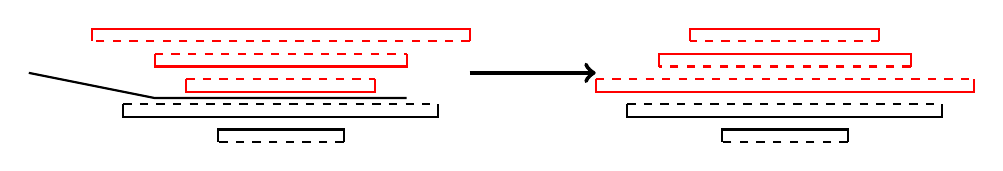
\begin{tikzpicture}[scale=0.8]

% \crepe{1cm}{0}{180};
% \crepe{1.5cm}{(0,1.5)}{0};
% \crepe{2cm}{(0,0)}{180};
% \crepe{2.5cm}{(0,1)}{0};
% \crepe{3cm}{(0,2)}{0};

\crepe{3cm}{4}{0}{1}{red};
\crepe{2cm}{3}{0}{0}{red};
\crepe{1.5cm}{2}{0}{0}{red};

% dessin de la pelle à tarte (une pelle à crêpes, ça n'existe pas ?)
\draw [color=black, thick, yshift=2*0.4cm, xshift=0cm,rotate=0*180] (-4,0.2) -- (-2,-0.2) -- (2,-0.2);

\crepe{2.5cm}{1}{0}{0}{black};
\crepe{1cm}{0}{0}{1}{black};

\draw [->,ultra thick,draw] (3,1) -- (5,1) ;

\crepe{1.5cm}{4}{8}{1}{red};
\crepe{2cm}{3}{8}{1}{red};
\crepe{3cm}{2}{8}{0}{red};
\crepe{2.5cm}{1}{8}{0}{black};
\crepe{1cm}{0}{8}{1}{black};


\end{tikzpicture}
